\chapter{Predicting susceptibility to tuberculosis based on gene expression profiling}\label{ch:comp}

\section[Abstract]{Abstract\footnotemark}


\footnotetext{Citation for chapter: Manuscript in Prep}

\section{Introduction}\label{ch03-introduction}

\section{Results}


\section{Discussion}


\section{Methods}



\clearpage


\subsection{Supplementary Figures}\label{ch03-supplementary-figures}

\begin{figure}[!htb]
\centering
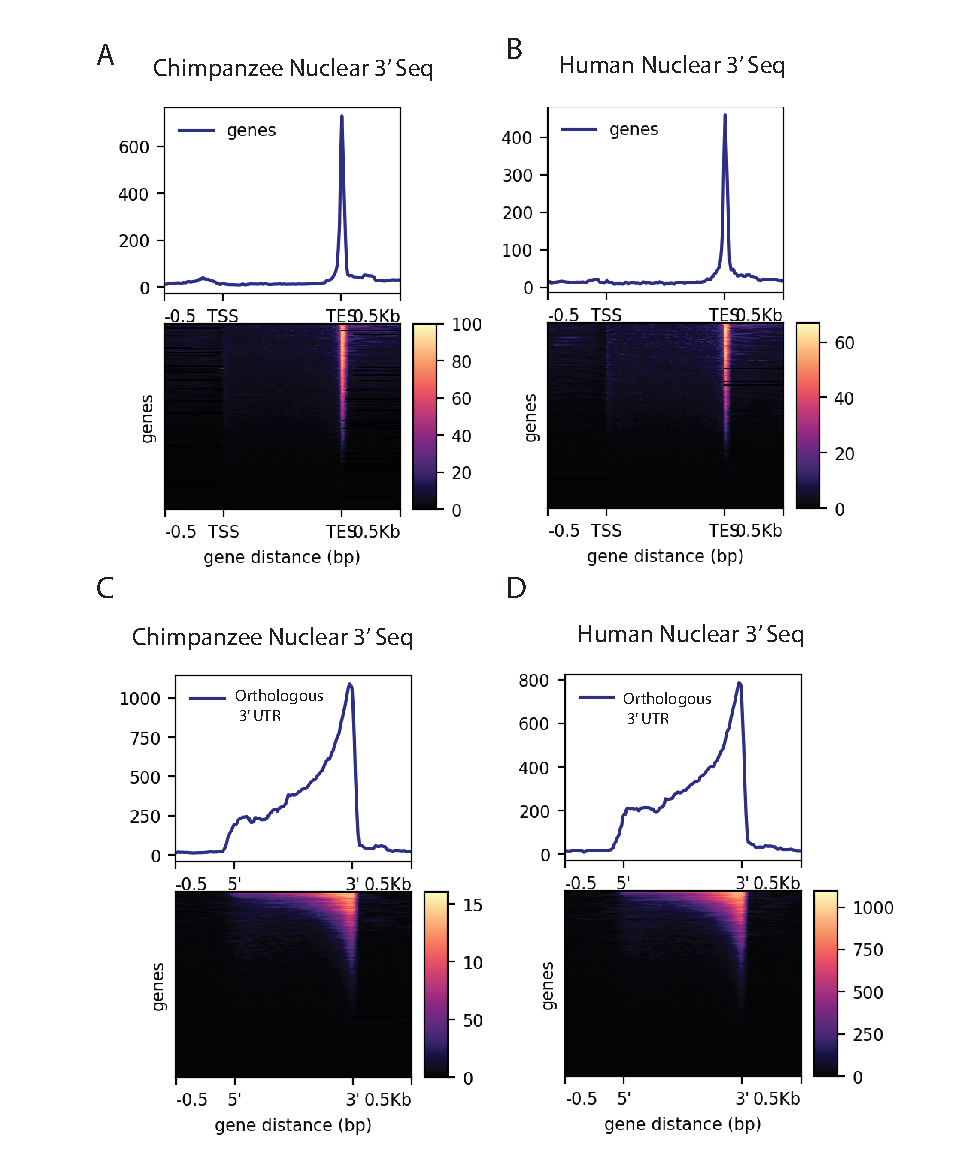
\includegraphics[width=5in]{img/ch03/Fig1-figSup1.pdf}
\caption[Density of merged human and chimpanzee 3' Seq]{\textbf{Density of merged human and chimpanzee 3' Seq} {\bf (A)}  Coverage of 6 chimpanzee, nuclear 3' seq reads along Refseq transcripts {\bf (B)}  Coverage of 5 human, nuclear 3'seq reads along Refseq transcripts {\bf (C)}  Coverage of 6 chimpanzee, nuclear 3' seq reads orthologous 3' UTRs {\bf (D)} Coverage of 5 human, nuclear 3' seq reads orthologous 3' UTRs}
\label{fig:ch03-deeptools}
\end{figure}
\clearpage

\begin{figure}[!htb]
\centering
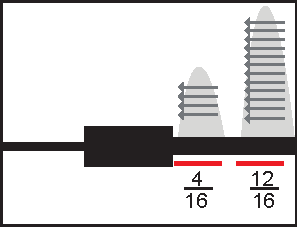
\includegraphics[width=5in]{img/ch03/Fig1-figSup2.pdf}
\caption[Model representation of usage calculation]{\textbf{Model representation of usage calculation} Representation of PAS usage calculation. Usage is a ratio of reads at each PAS to the number of reads mapping to any PAS in the same gene. Adapted from Chapter \ref{ch:QTL}}
\label{fig:ch03-UsageCalc}
\end{figure}
\clearpage

\begin{figure}[!htb]
\centering
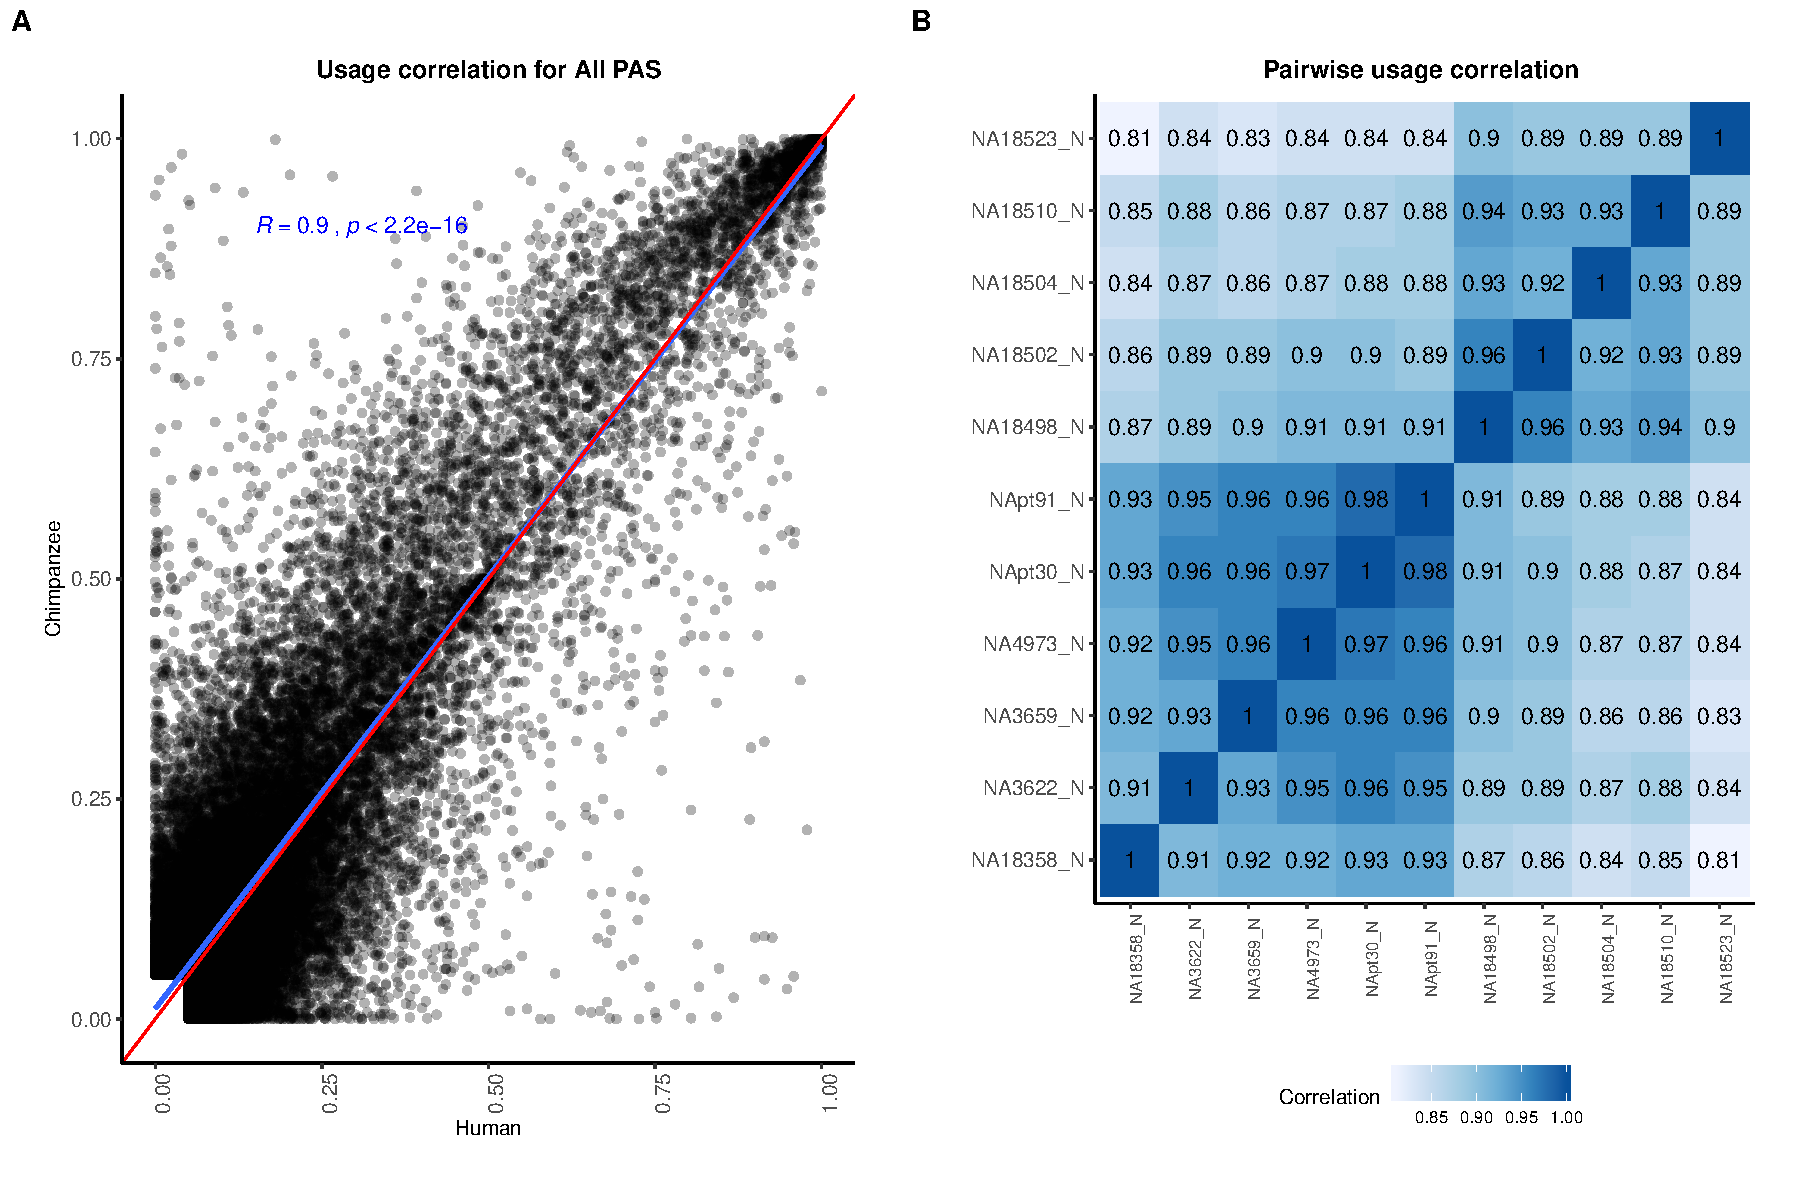
\includegraphics[width=5in]{img/ch03/Fig1-figSup3.pdf}
\caption[PAS usage is highly correlated across species]{\textbf{PAS usage is highly correlated across species} {\bf (A)}  Correlation between human and chimpanzee PAS usage for 44,432 PAS. Red line is a 1:1 line. Linear regression line and Pearson's correlation plotted in blue. {\bf (B)}  Pairwise correlation for human and chimpanzee PAS usage.}
\label{fig:ch03-UsageCorr}
\end{figure}
\clearpage

\begin{figure}[!htb]
\centering
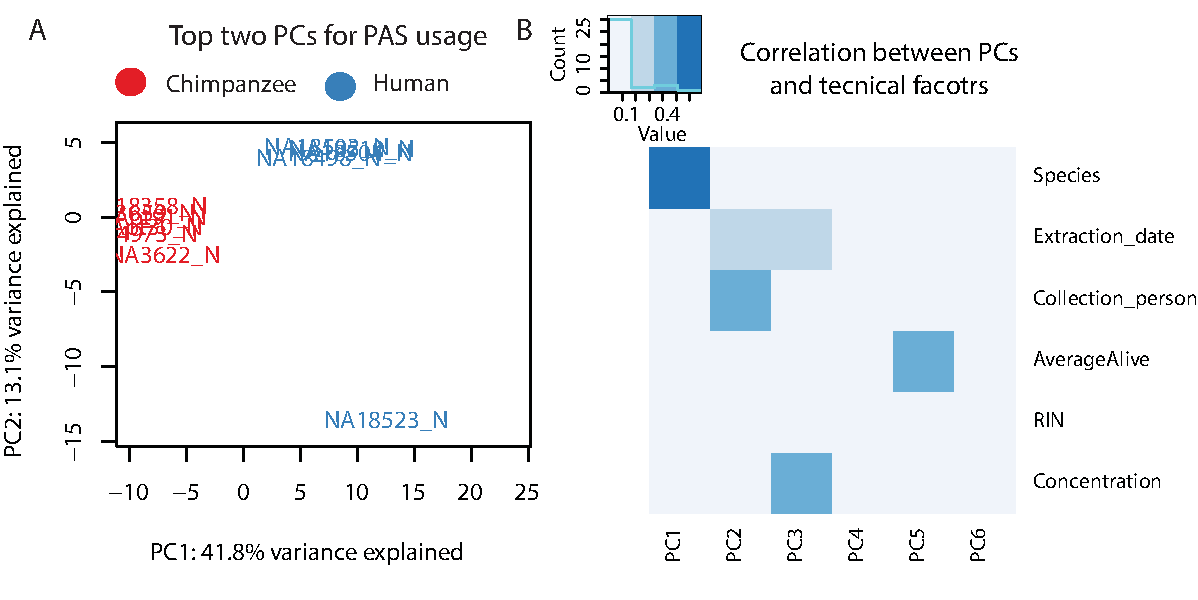
\includegraphics[width=5in]{img/ch03/Fig1-figSup4.pdf}
\caption[Variation in PAS usage]{\textbf{Variation in PAS usage} {\bf (A)}  Plot of first two principal components \emph{(PCs)} calculated by a principal component analysis on PAS usage (44,432 PAS). Chimpanzee samples are shown in red and human samples are shown in blue {\bf (B)}  Heatmap representing correlation between technical factors and PCs. Y axis factors include: Species, Extraction date, Collection person, AverageAlive (average of two live dead calculations at time of collection), RIN score, RNA concentration. Explanation of factors and values in supplemental table \ref{tab:ch03-s1}}
\label{fig:ch03-PCAthreeprime}
\end{figure}
\clearpage

\begin{figure}[!htb]
\centering
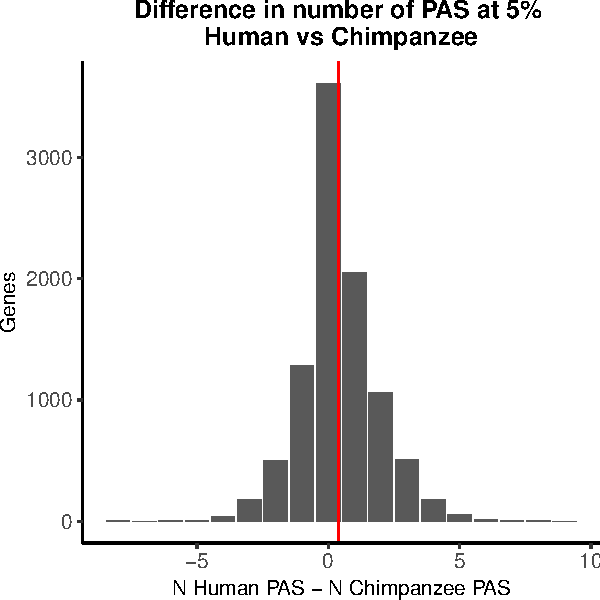
\includegraphics[width=5in]{img/ch03/Fig1-figSup6.pdf}
\caption[Number of PAS per gene largely conserved between species]{\textbf{Number of PAS per gene largely conserved between species} Histogram of the number of PAS detected at 5\% usage in human minus the number of 5\% usage in chimpanzees. Red vertical line represents mean difference (0.39).}
\label{fig:ch03-SpecPASnum}
\end{figure}
\clearpage


\begin{figure}[!htb]
\centering
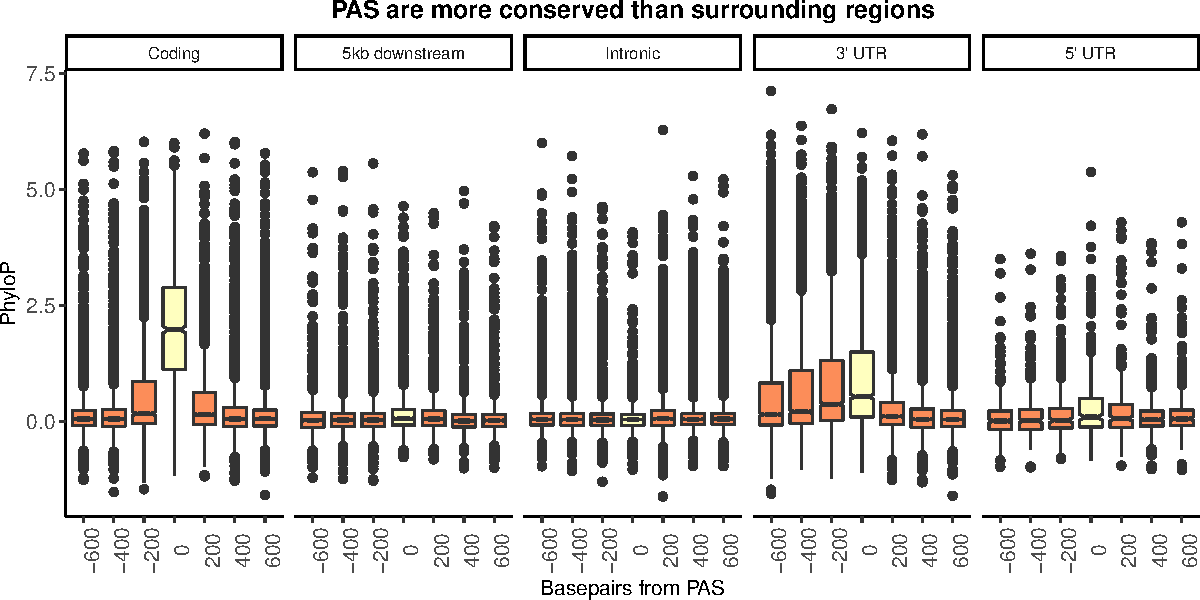
\includegraphics[width=5in]{img/ch03/Fig1-figSup7.pdf}
\caption[Figure 1B separated by genic location]{\textbf{Figure 1B separated by genic location} Mean PhyloP scores for PAS regions (yellow) and 200 base pair bins upstream and downstream of PAS (orange). A one-sided Wilcoxon test was used to test for increased PhyloP in PAS regions  (Coding region: $p < 2.2x10^{-16}$, 5 kb downstream of genes: $p = 7.02x10^{-6}$, intron: $p=0.99$, 3' UTR: $p < 2.2x10^{-16}$, 5' UTR: $p = 0.011$).}
\label{fig:ch03-phylopLoc}
\end{figure}
\clearpage

\begin{figure}[!htb]
\centering
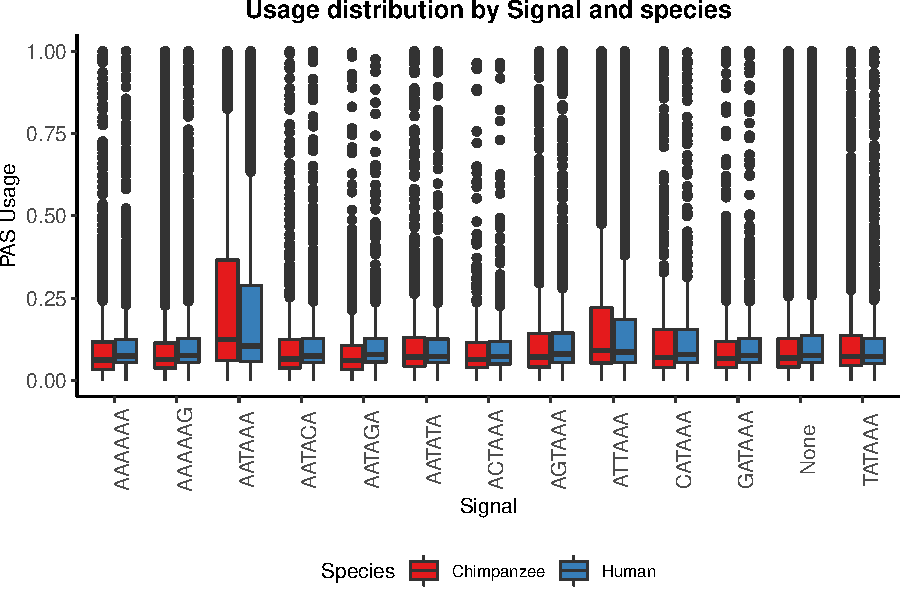
\includegraphics[width=5in]{img/ch03/Fig1-figSup8.pdf}
\caption[PAS with AATAAA and ATTAAA are used more often]{\textbf{PAS with AATAAA and ATTAAA are used more often} Mean PAS usage of the top two signal site motifs in human and chimpanzee plotted by annotated signal site.}
\label{fig:ch03-SignalUsage}
\end{figure}
\clearpage

\begin{figure}[!htb]
\centering
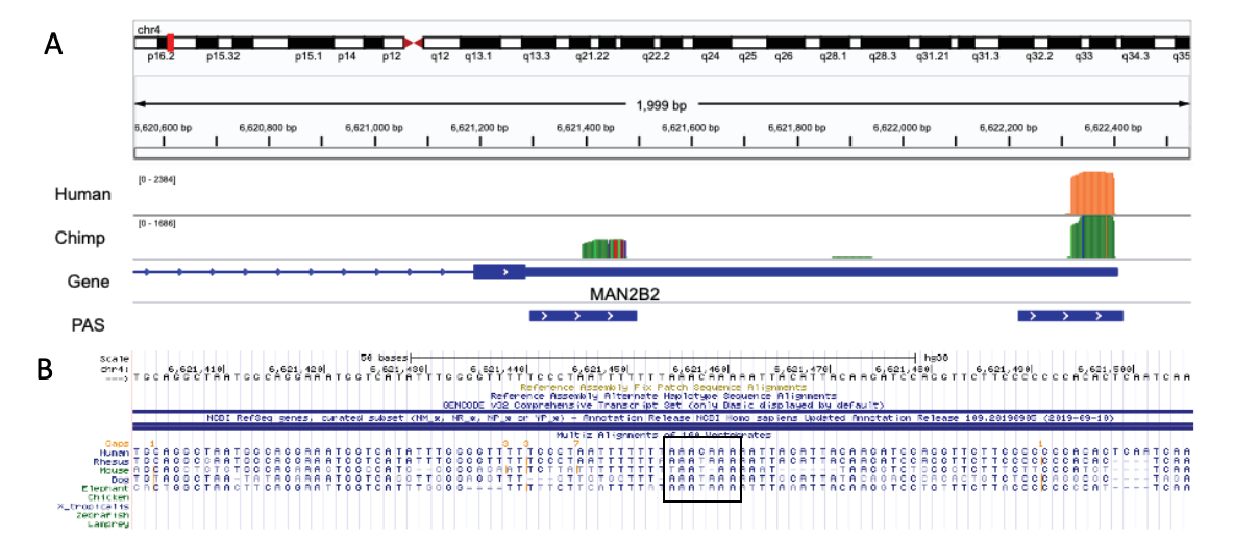
\includegraphics[width=5in]{img/ch03/Fig1_figSup9.pdf}
\caption[Chimp specific PAS likely due to loss of signal site in human lineage]{\textbf{Chimp specific PAS likely due to loss of signal site in human lineage} {\bf (A)} IGV track for example of a chimpanzee specific PAS in MAN2B2 gene. Top track is merged coverage from 5 human nuclear 3' seq libraries. Chimp track is merged coverage from 6 chimpanzee nuclear 3' seq libraries lifted to human genome with CrossMap\citep{zhao_crossmap_2014} {\bf (B)}  Sequence alignment for region upstream of proximal PAS from UCSC genome browser\citep{kent_human_2002}. Black box indicates the signal site location. Canonical signal site is the ancestral state and was lost in the human lineage.}
\label{fig:ch03-exChimpspec}
\end{figure}
\clearpage

\begin{figure}[!htb]
\centering
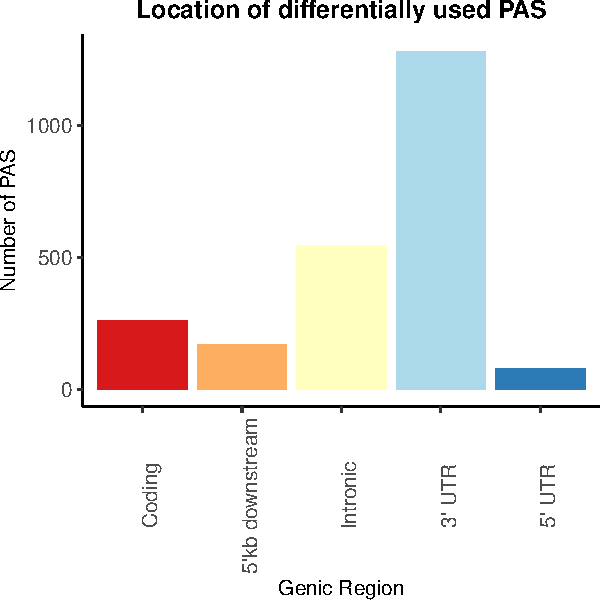
\includegraphics[width=5in]{img/ch03/Fig2-figSup1.pdf}
\caption[Genic Location of PAS differentially used between human and chimpanzee]{\textbf{Genic Location of PAS differentially used between human and chimpanzee} Differentially used PAS (5\% FDR) between human chimpanzee by genic annotation.}
\label{fig:ch03-dPAS}
\end{figure}
\clearpage

\begin{figure}[!htb]
\centering
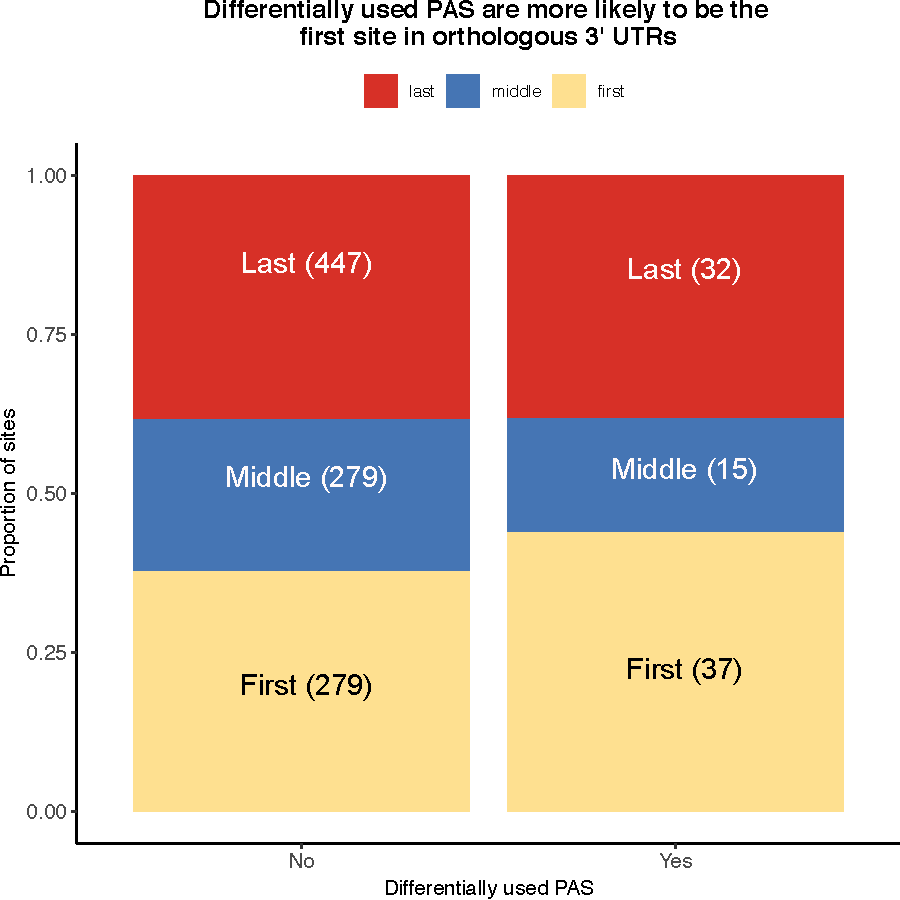
\includegraphics[width=5in]{img/ch03/Fig2-figSup2.pdf}
\caption[Location of PAS within Orthologous 3' UTRs]{\textbf{Location of PAS within Orthologous 3' UTRs}Proportion of sites differentially used or conserved by whether they are the first (yellow), middle (blue), or last PAS (red) in orthologous exons. }
\label{fig:ch03-whichUTR}
\end{figure}
\clearpage

\begin{figure}[!htb]
\centering
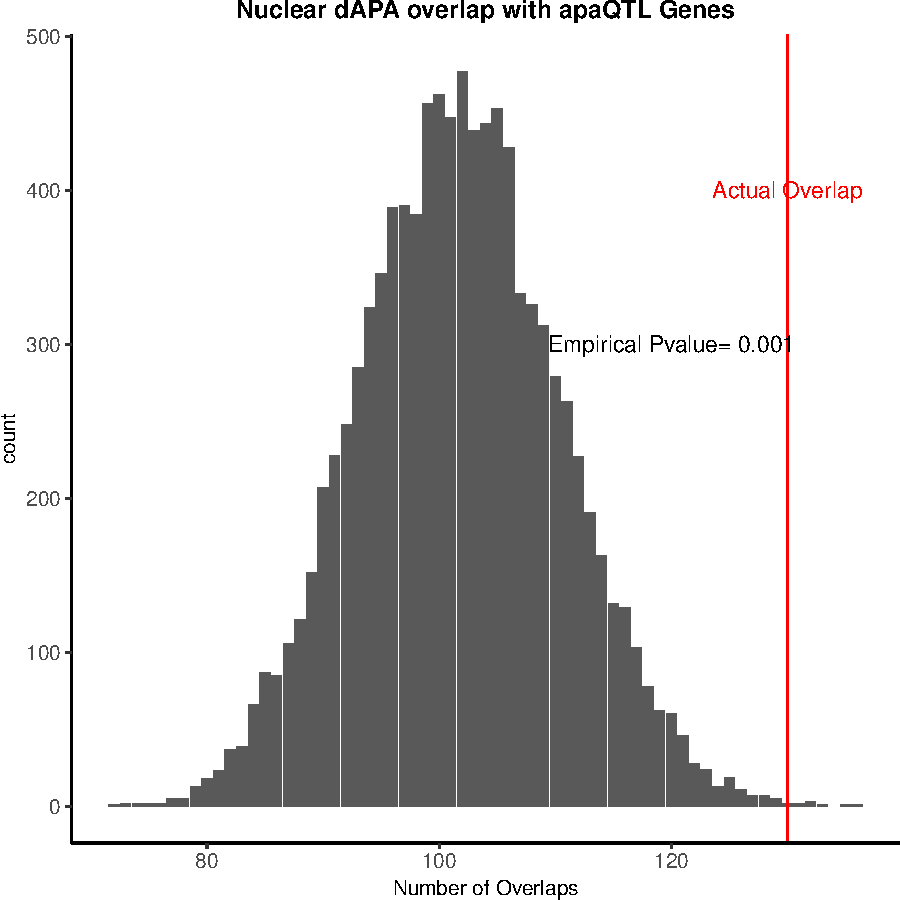
\includegraphics[width=5in]{img/ch03/Fig2_figSup3.pdf}
\caption[Genes with differentially used PAS are enriched for genes with apaQTL ]{\textbf{Genes with differentially used PAS are enriched for genes with apaQTL} 10,000 random subsamples of genes tested for differential APA and overlap with genes with apaQTLs from Chapter \ref{ch:QTL}. Red line represents the actual overlap between genes with differential usage of at least one PAS and apaQTL genes.}
\label{fig:ch03-dPASQTL}
\end{figure}
\clearpage

\begin{figure}[!htb]
\centering
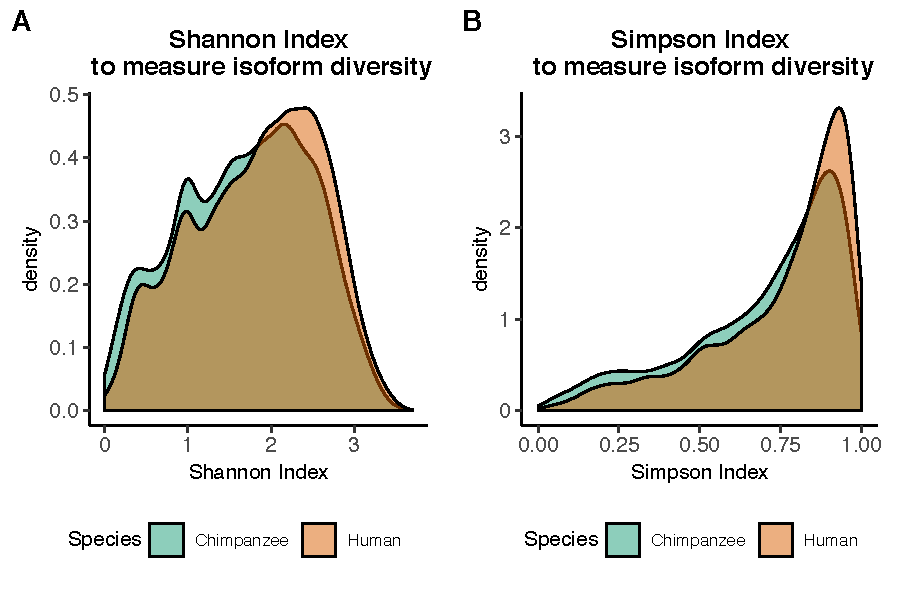
\includegraphics[width=5in]{img/ch03/Fig2-figSup4.pdf}
\caption[Information content measurement densities]{\textbf{Information content measurement densities} {\bf (A)}  Density of Shannon indices for all tested genes in human and chimpanzee ( $- \sum_{i=1}^{S} p_{i}log_{2}p_{i}$ ) {\bf (B)}  Density of Simpson indices for all tested genes in human and chimpanzee ($1 - \sum_{i=1}^{S} p^{2}_{i}$)  }
\label{fig:ch03-bothDensities}
\end{figure}
\clearpage


\begin{figure}[!htb]
\centering
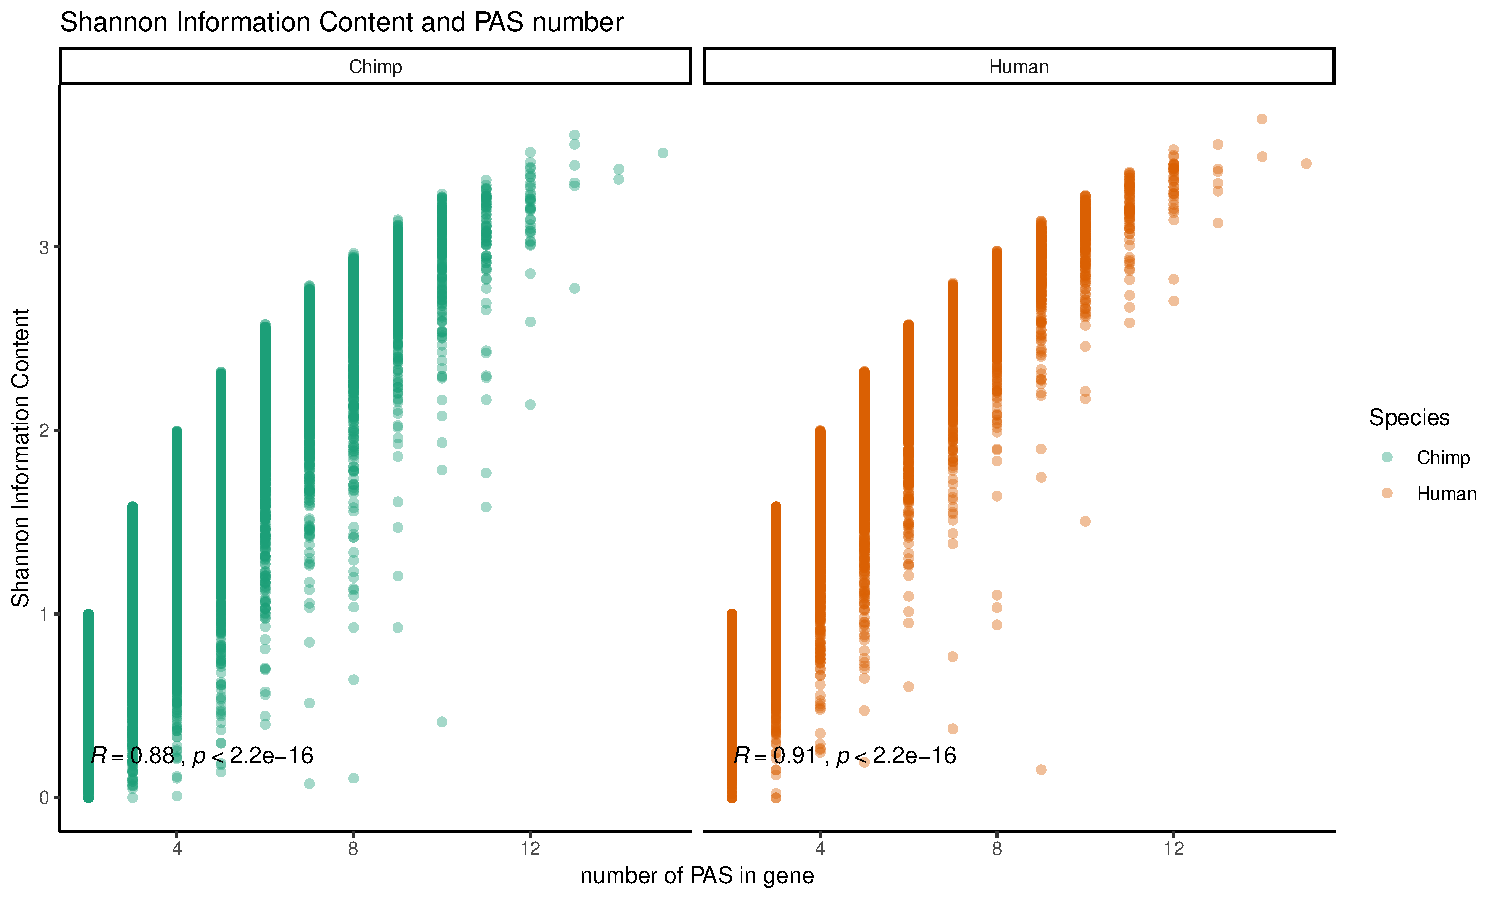
\includegraphics[width=5in]{img/ch03/Fig2-figSup5.pdf}
\caption[Relationship between Shannon index and PAS number ]{\textbf{Relationship between Shannon index and PAS number} Shannon information index plotted against the number of PAS detect for each gene. Pearson's correlation and significance in black. }
\label{fig:ch03-shanonNum}
\end{figure}
\clearpage

\begin{figure}[!htb]
\centering
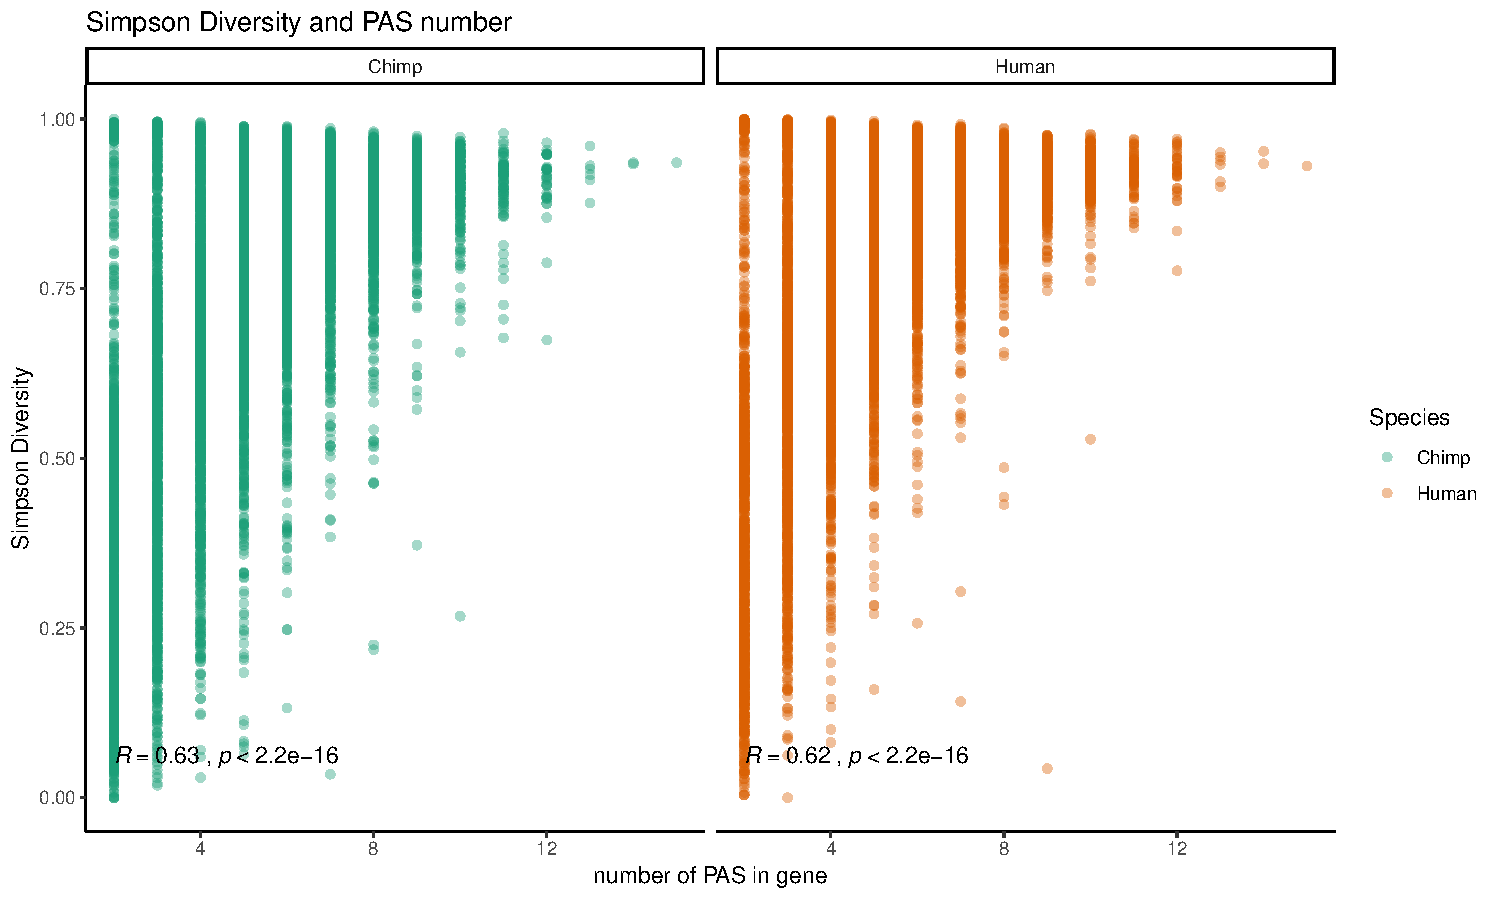
\includegraphics[width=5in]{img/ch03/Fig2-figSup6.pdf}
\caption[Relationship between Simpson diversity index and PAS number]{\textbf{Relationship between Simpson diversity index and PAS number} Simpson's diversity index plotted against the number of PAS detect for each gene. Pearson?s correlation and significance in black.}
\label{fig:ch03-simpNum}
\end{figure}
\clearpage

\begin{figure}[!htb]
\centering
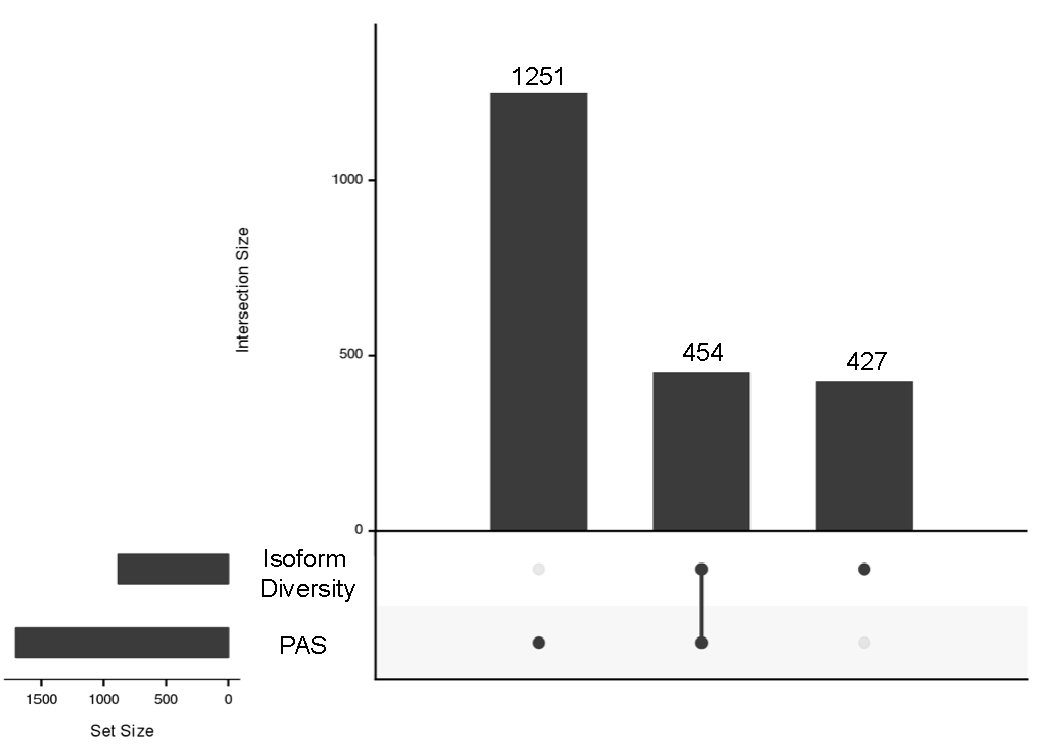
\includegraphics[width=5in]{img/ch03/Fig2_figSup7.pdf}
\caption[Intersection between genes with PAS and isoform diversity differences]{\textbf{Intersection between genes with PAS and isoform diversity differences} 1251 genes have significant differences in PAS usage at between human and chimpanzee (left). 454 genes have significant differences in APA between humans and chimpanzee in PAS usage and in isoform diversity (middle). 427 genes with differences in isoform diversity level only (right).}
\label{fig:ch03-simpNum}
\end{figure}
\clearpage

\begin{figure}[!htb]
\centering
\includegraphics[width=5in]{img/ch03/Fig3-figSup1.pdf}
\caption[Figure 3 relationships expanded to total usage]{\textbf{Figure 3 relationships expanded to total usage} {\bf (A)}  Total mRNA  $\Delta PAU$ for top intronic or 3' UTR PAS per gene plotted against differential effect size from differential expression analysis. {\bf (B)} Total mRNA $\Delta PAU$ for top intronic or 3' UTR PAS per gene plotted against differential effect size from differential expression analysis for genes with significant differences in each phenotype at 5\% FDR. {\bf (C)} Total mRNA $\Delta PAU$ for top intronic or 3' UTR PAS per gene plotted against differential effect size from differential expression analysis. {\bf (D)} Total mRNA $\Delta PAU$ for top intronic or 3' UTR PAS per gene plotted against differential effect size from differential expression analysis for genes with significant differences in each phenotype at 5\% FDR. In all panels, I calculated the linear regression and pearson's correlation with the r package ggpubr. In B and D, I  colored the points and regression line by genic location. In all panels, negative $\Delta PAU$ and DE effect sizes represent upregulation in chimpanzees.}
\label{fig:ch03-totalDPASDE}
\end{figure}
\clearpage

\begin{figure}[!htb]
\centering
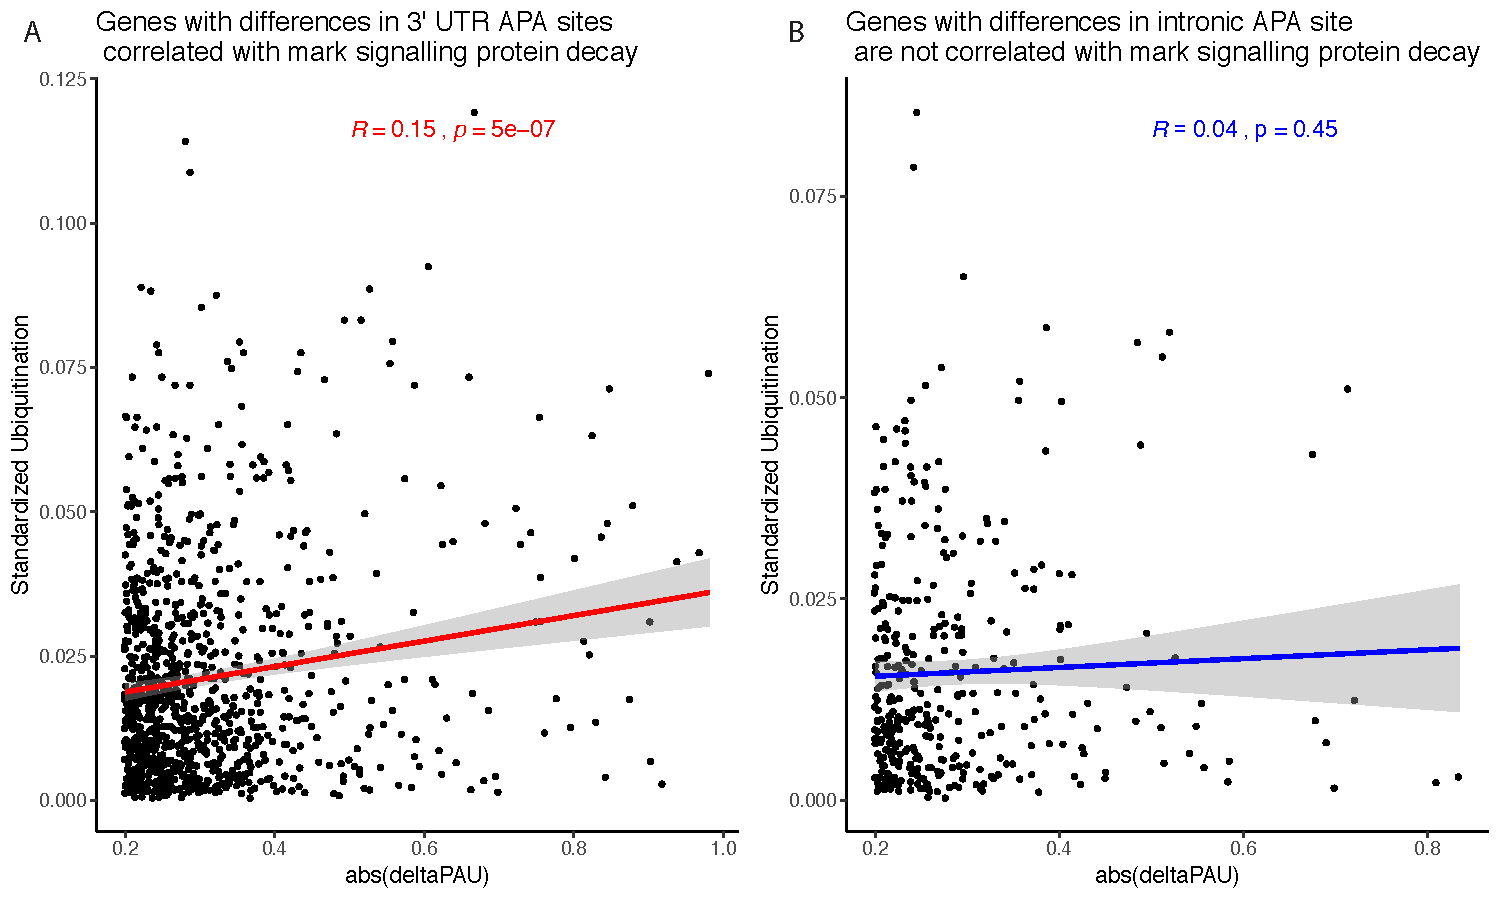
\includegraphics[width=5in]{img/ch03/Fig3-figSup2.pdf}
\caption[Relationship between APA differences and protein decay mark]{\textbf{Relationship between APA differences and protein decay mark} {\bf (A)} Absolute value of $\Delta PAU$ for 3' UTR PAS with significant difference at site level plotted against the number of ubiquitination marks in the gene standardized by the number of amino acids. Regression line and Pearson's correlation are plotted in red.{\bf (B)} Absolute value of $\Delta PAU$ for intronic PAS with significant difference at site level plotted against the number of ubiquitination marks in the gene standardized by the number of amino acids. Regression line and Pearson?s correlation are plotted in blue.}
\label{fig:ch03-ubiq}
\end{figure}
\clearpage

\begin{figure}[!htb]
\centering
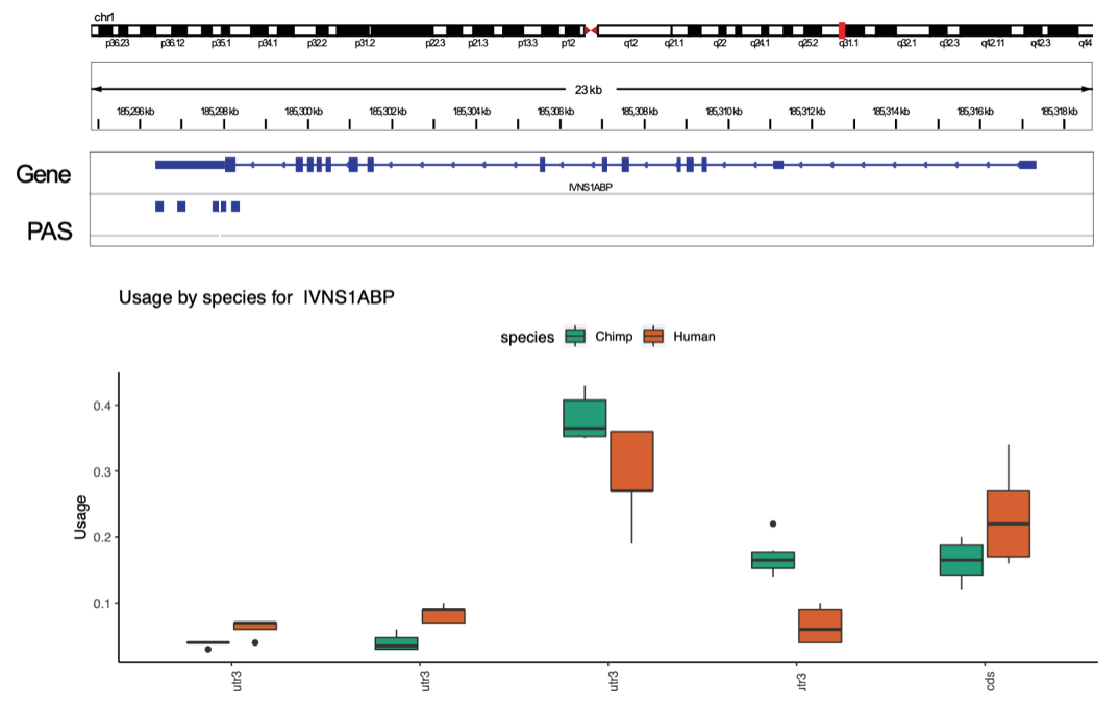
\includegraphics[width=5in]{img/ch03/Fig4_figSup1.pdf}
\caption[Gene with significant differences in isoform diversity only]{\textbf{Gene with significant differences in isoform diversity only} Human and chimpanzee usage for 5 PAS identified in the IVNS1ABP gene. None of the PAS measured have significant differences in usage at 5\% FDR. IVNS1ABP is not differentially expressed.}
\label{fig:ch03-ivn}
\end{figure}
\clearpage

\begin{figure}[!htb]
\centering
\includegraphics[width=5in]{img/ch03/Fig4-figSup2.pdf}
\caption[Relationship between $\Delta PAU$  and differential translation effect sizes]{\textbf{Relationship between $\Delta PAU$  and differential translation effect sizes} {\bf (A)} $\Delta PAU$ for top 3' UTR and intronic PAS plotted against differential translation \emph{(TE)} effect size as reported by Wang \emph{et al.}\citep{wang_post-translational_2018} {\bf (B)} $\Delta PAU$ for top 3' UTR and intronic PAS plotted against TE effect size as reported by Wang \emph{et al.} \citep{wang_post-translational_2018} separated by genic location.  {\bf (C)} $\Delta PAU$ for top 3' UTR and intronic PAS with significant differences in usage plotted against TE effect size for significant genes (5\% FWER) as reported by Wang \emph{et al.}\citep{wang_post-translational_2018}. {\bf (D)}  $\Delta PAU$ for top 3' UTR and intronic PAS with significant differences in usage plotted against TE effect size for significant genes (5\% FWER) as reported by Wang \emph{et al.}\citep{wang_post-translational_2018} separated by genic location. Linear regression line was plotted and Pearson's correlation was calculated for data in each panel.}
\label{fig:ch03-TEdAPA}
\end{figure}
\clearpage

\begin{figure}[!htb]
\centering
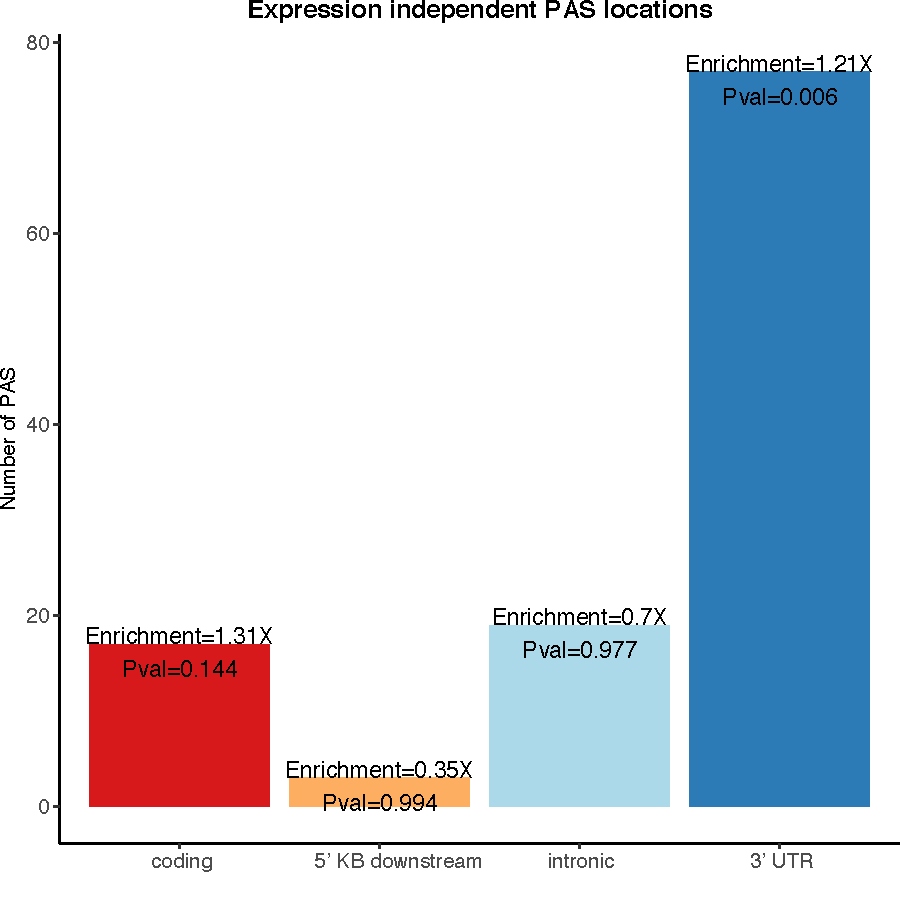
\includegraphics[width=5in]{img/ch03/Fig6-figSup1.pdf}
\caption[Enrichment for 3' UTR PAS in genes differentially expressed in protein and not in mRNA]{\textbf{Enrichment for 3' UTR PAS in genes differentially expressed in protein and not in mRNA} Genic location enrichments for the PAS in genes differentially expressed at protein level but not mRNA level among all differentially used PAS. Pvalues were calculated with a hypergeometric test.}
\label{fig:ch03-dpnotE}
\end{figure}
\clearpage


\begin{figure}[!htb]
\centering
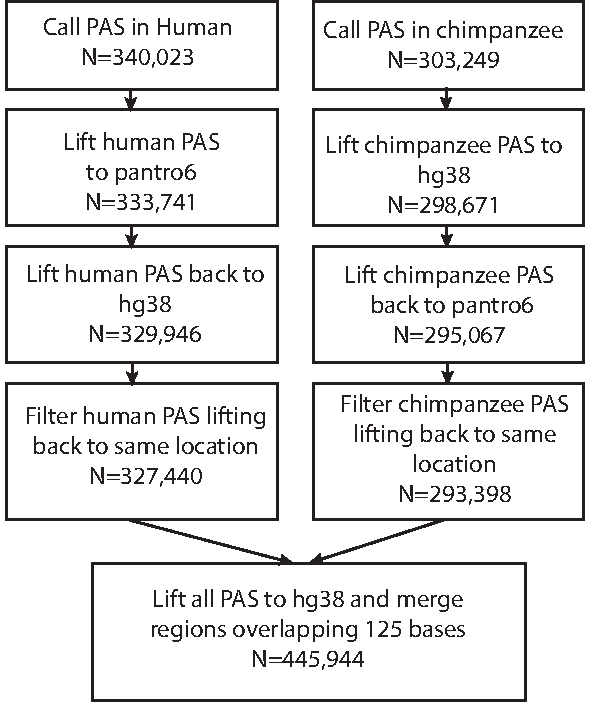
\includegraphics[width=5in]{img/ch03/Fig1_figSup10.pdf}
\caption[Reciprocal liftover pipeline]{\textbf{Reciprocal liftover pipeline} Reciprocal liftover pipeline for unfiltered PAS including the number of sites remaining at each step. Liftover using UCSC liftover tool and chain files downloaded from UCSC genome browser \citep{kent_human_2002}. }
\label{fig:ch03-liftover}
\end{figure}
\clearpage

\begin{figure}[!htb]
\centering
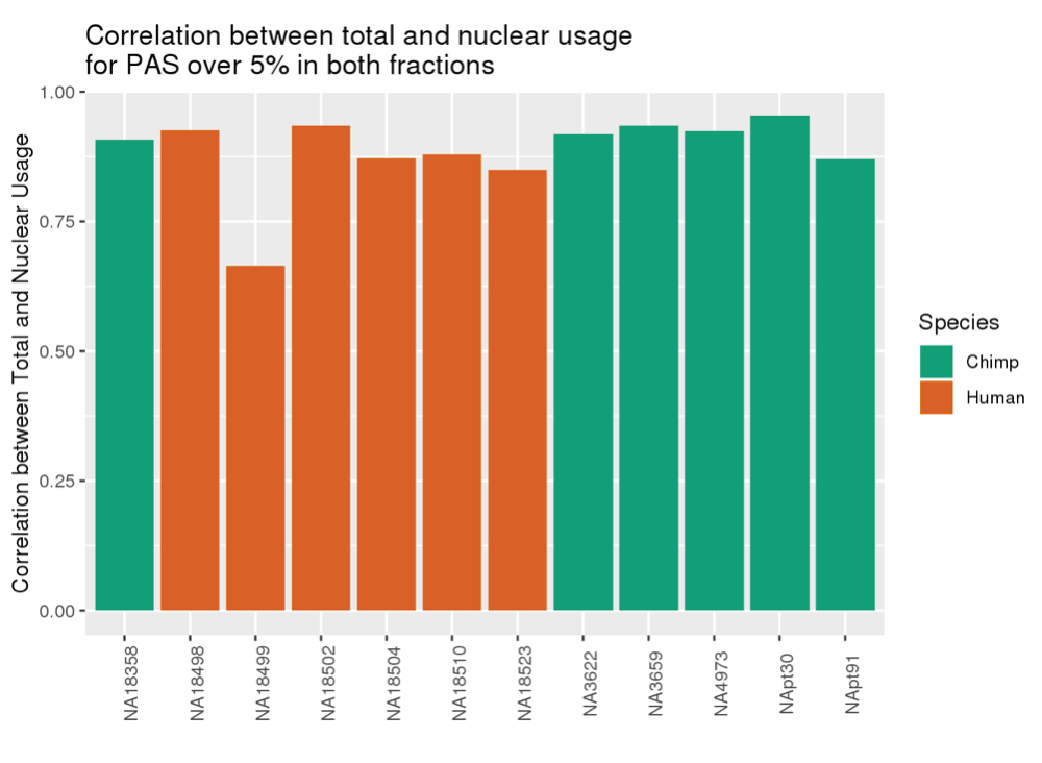
\includegraphics[width=5in]{img/ch03/Fig1_figSup11.pdf}
\caption[NA18499 removed from analysis due to low correlation between fractions]{\textbf{NA18499 removed from analysis due to low correlation between fractions} Pearson's correlation between PAS usage calculated using nuclear 3' seq libraries and total mRNA 3' seq libraries, calculated using sites reaching 5\% in one species in both fractions. (Plot from previous commit 30ff122 on Aril 9, 2020). }
\label{fig:ch03-removeInd}
\end{figure}
\clearpage

\begin{figure}[!htb]
\centering
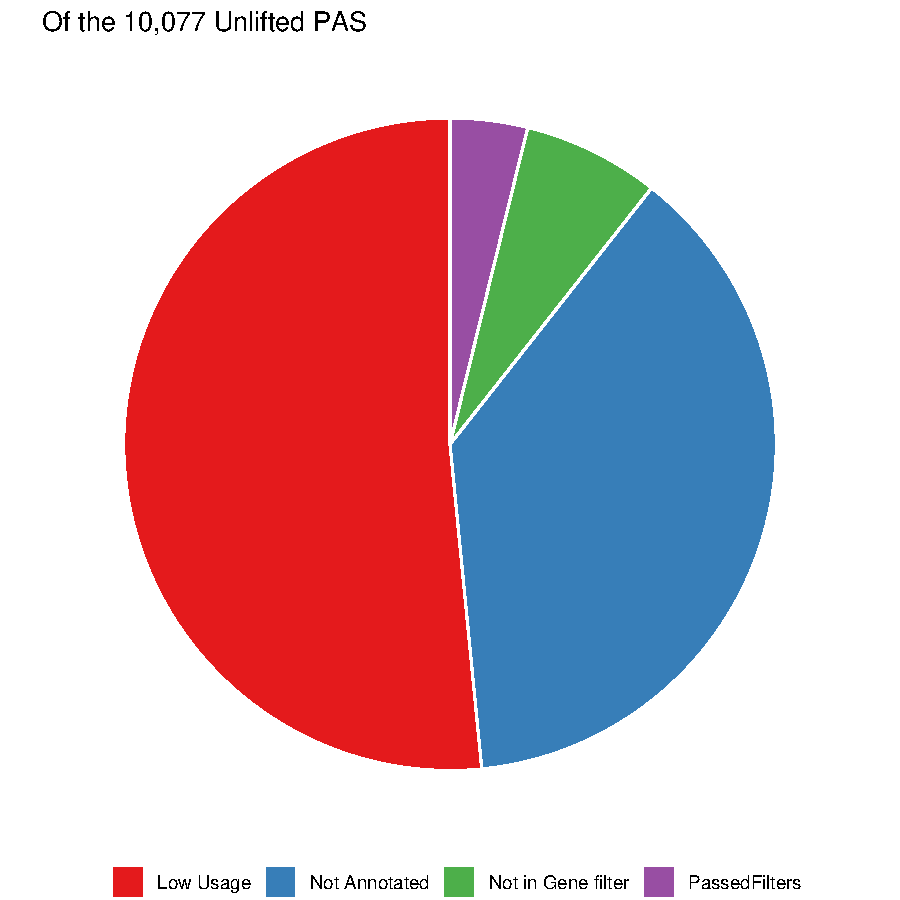
\includegraphics[width=5in]{img/ch03/Fig2-figSup8.pdf}
\caption[PAS that do not lift from human to chimp]{\textbf{PAS that do not lift from human to chimp} Of the 10,077 PAS that do not reciprocally lift from human to chimp, distribution of where sites are filtered out. Most are lost due to not mapping to genes or due to low usage (likely noise). }
\label{fig:ch03-unlift}
\end{figure}
\clearpage

\begin{figure}[!htb]
\centering
\includegraphics[width=5in]{img/ch03/Fig3-figSup3.pdf}
\caption[Figure 3 without genes affected by liftover]{\textbf{Figure 3 without genes affected by liftover} {\bf (A)} $\Delta PAU$ for top intronic or 3' UTR PAS per gene plotted against differential effect size from differential expression analysis.  {\bf (B)}  $\Delta PAU$ for top intronic or 3' UTR PAS per gene plotted against differential effect size from differential expression analysis for genes with significant differences in each phenotype at 5\% FDR. {\bf (C)}  $\Delta PAU$ for top intronic or 3' UTR PAS per gene plotted against differential effect size from differential expression analysis. {\bf (D)}  $\Delta PAU$ for top intronic or 3' UTR PAS per gene plotted against differential effect size from differential expression analysis for genes with significant differences in each phenotype at 5\% FDR. In all panels, I calculated the linear regression and pearson's correlation with the r package ggpubr. In B and D, I  colored the points and regression line by genic location. In all panels, negative $\Delta PAU$ and DE effect sizes represent upregulation in chimpanzees.}
\label{fig:ch03-unliftfig3}
\end{figure}
\clearpage



\begin{figure}[!htb]
\centering
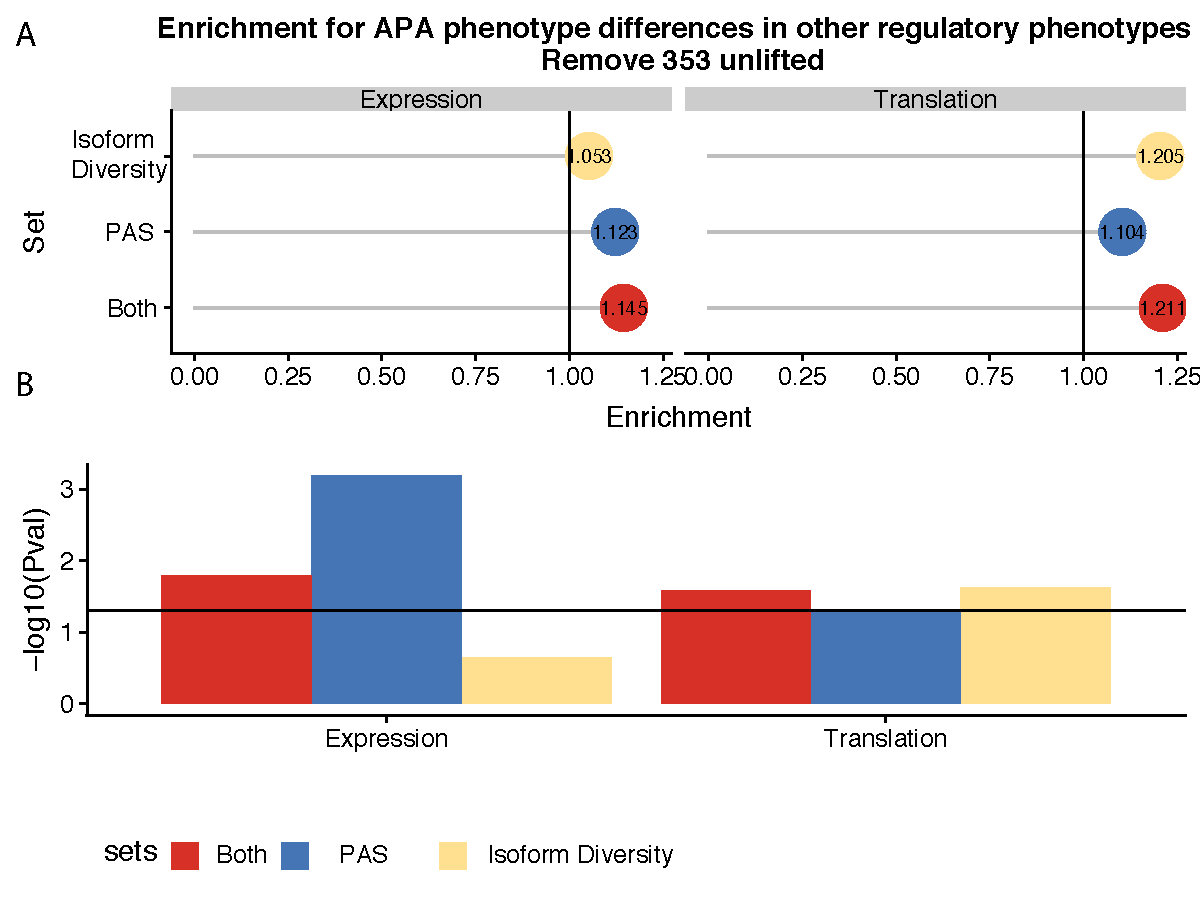
\includegraphics[width=5in]{img/ch03/Fig4-figSup3.pdf}
\caption[Figure 4 without genes affected by liftover]{\textbf{Figure 4 without genes affected by liftover} {\bf (A)} Enrichment of genes with differences in isoform diversity, PAS usage, or both within differential expressed genes and differentially translated genes after removing genes likely affected by liftover. Differentially translated genes reported by Wang \emph{et al.}\citep{wang_post-translational_2018}. {\bf (B)}  $-log_{10}(p-values)$ for enrichments in A calculated with hypergeometric tests. Horizontal line represents $p= 0.05$.}
\label{fig:ch03-unliftfig4}
\end{figure}
\clearpage


\begin{figure}[!htb]
\centering
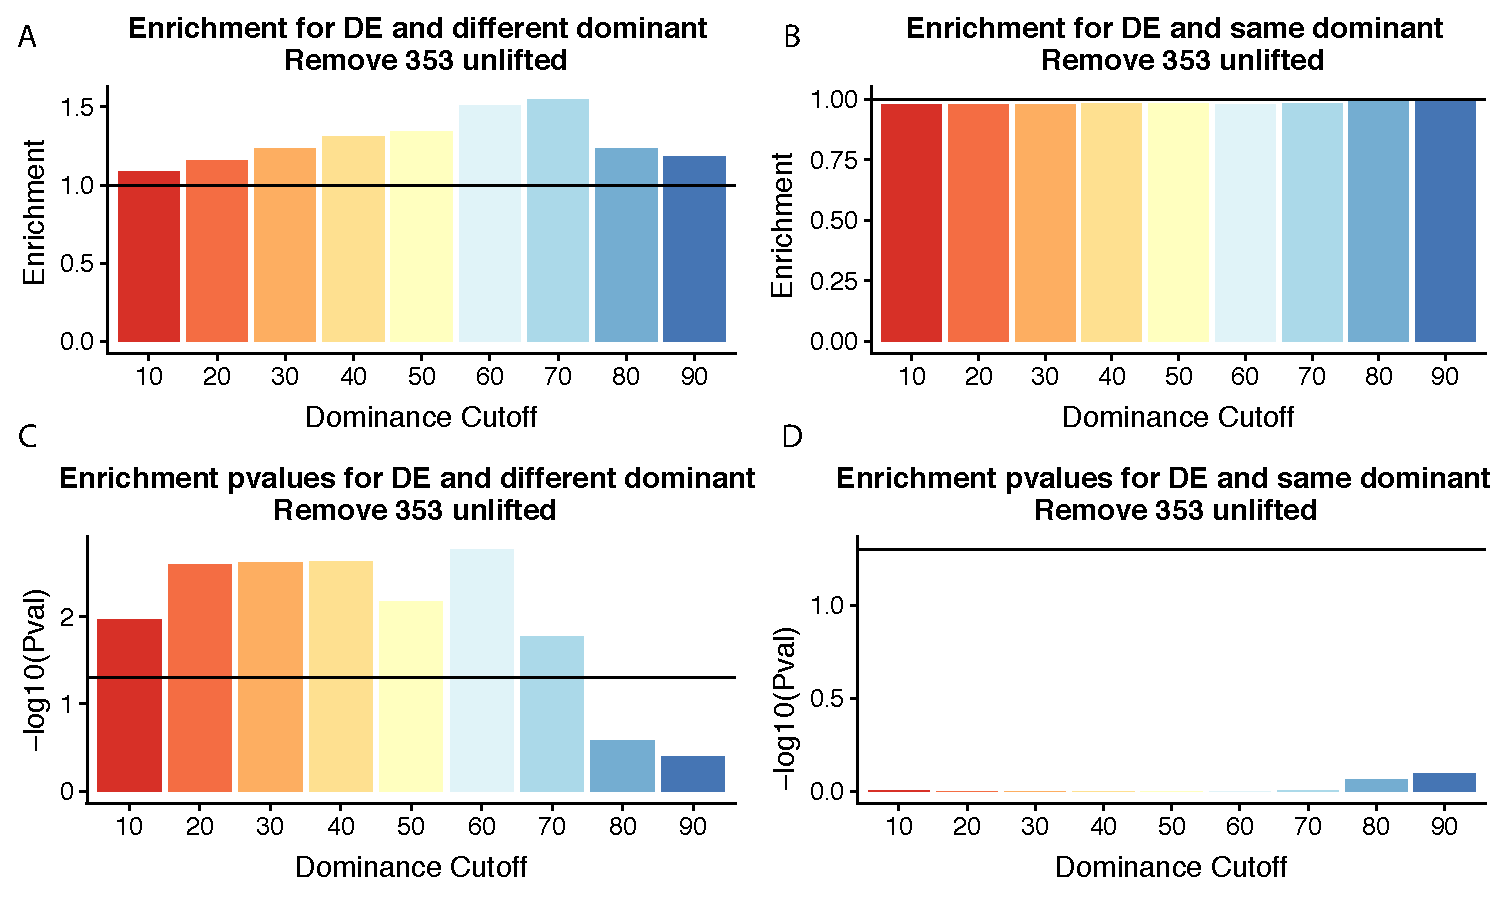
\includegraphics[width=5in]{img/ch03/Fig5-figSup1.pdf}
\caption[Figure 5 without genes affected by liftover]{\textbf{Figure 5 without genes affected by liftover} {\bf (A)}  Enrichment of genes with the different (left) or same (right) dominant PAS by dominant cutoff in differentially expressed genes after removing genes likely affected by liftover. {\bf (B)} $-log_{10}(p-values)$ for enrichments in A calculated with hypergeometric tests. Horizontal line represents $p= 0.05$.}
\label{fig:ch03-unliftfig4}
\end{figure}
\clearpage

\begin{figure}[!htb]
\centering
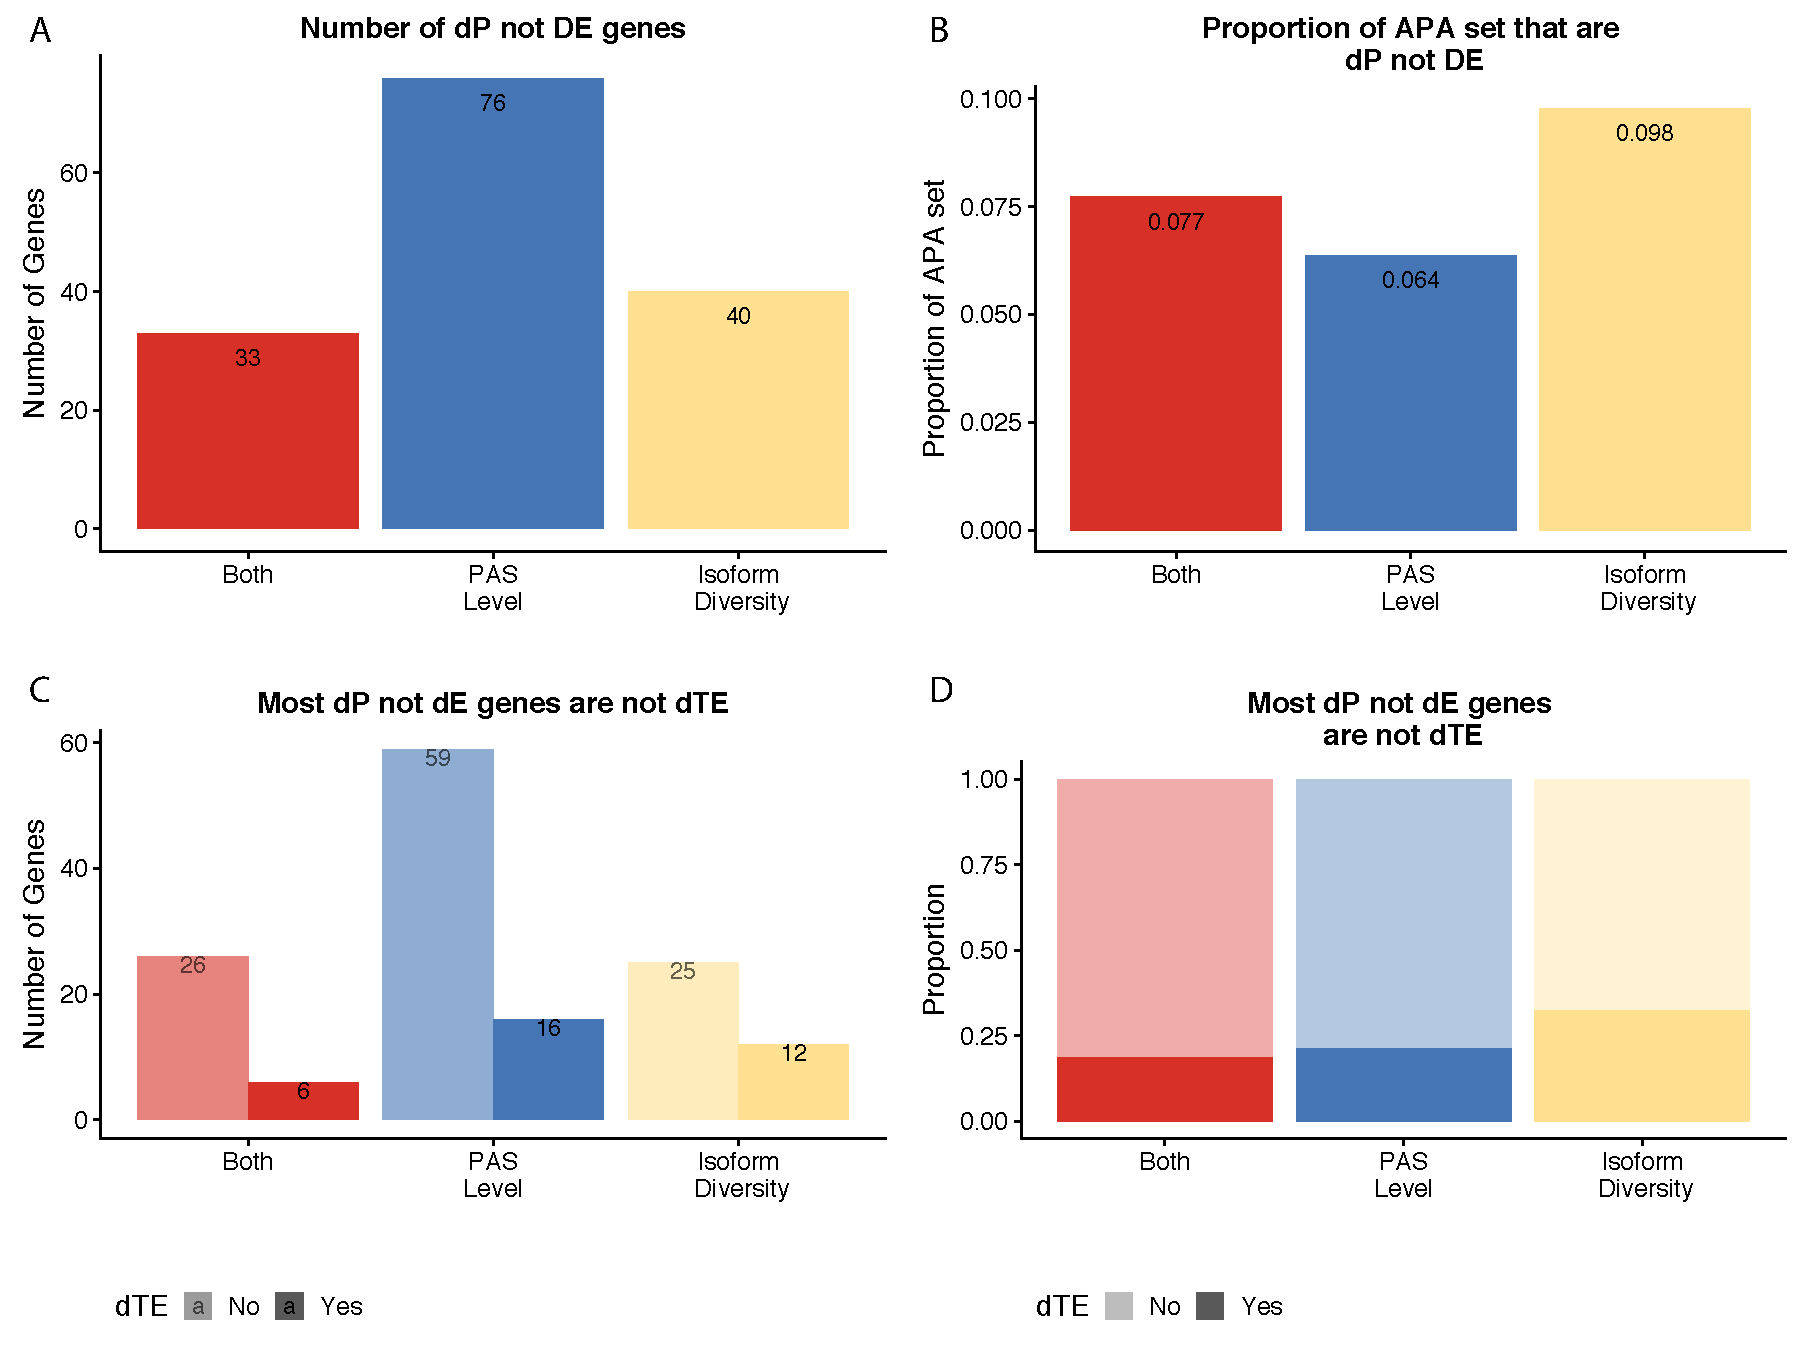
\includegraphics[width=5in]{img/ch03/Fig6-figSup2.pdf}
\caption[Figure 6 without genes affected by liftover]{\textbf{Figure 6 without genes affected by liftover} {\bf (A)} Number of genes with differences in isoform diversity, PAS usage or both differentially expressed in protein (5\% FDR) but not in mRNA (5\% FDR). Genes differentially expressed in protein from Khan \emph{et al.}\citep{khan_primate_2013} {\bf (B)} Proportion of genes with differential isoform diversity, PAS usage or both that are differentially expressed in protein (5\% FDR), but not mRNA (5\% FDR). {\bf (C)} Genes reported in separated by genes differentially translated at 5\% FDR. Differentially translated gene reported in Wang \emph{et al.}\citep{wang_post-translational_2018}. {\bf (D)} Genes differentially expressed in protein but not in mRNA, colored by differences in APA. Proportion of genes in the set differentially translated at 5\% FDR.}
\label{fig:ch03-unliftfig6}
\end{figure}
\clearpage


\begin{figure}[!htb]
\centering
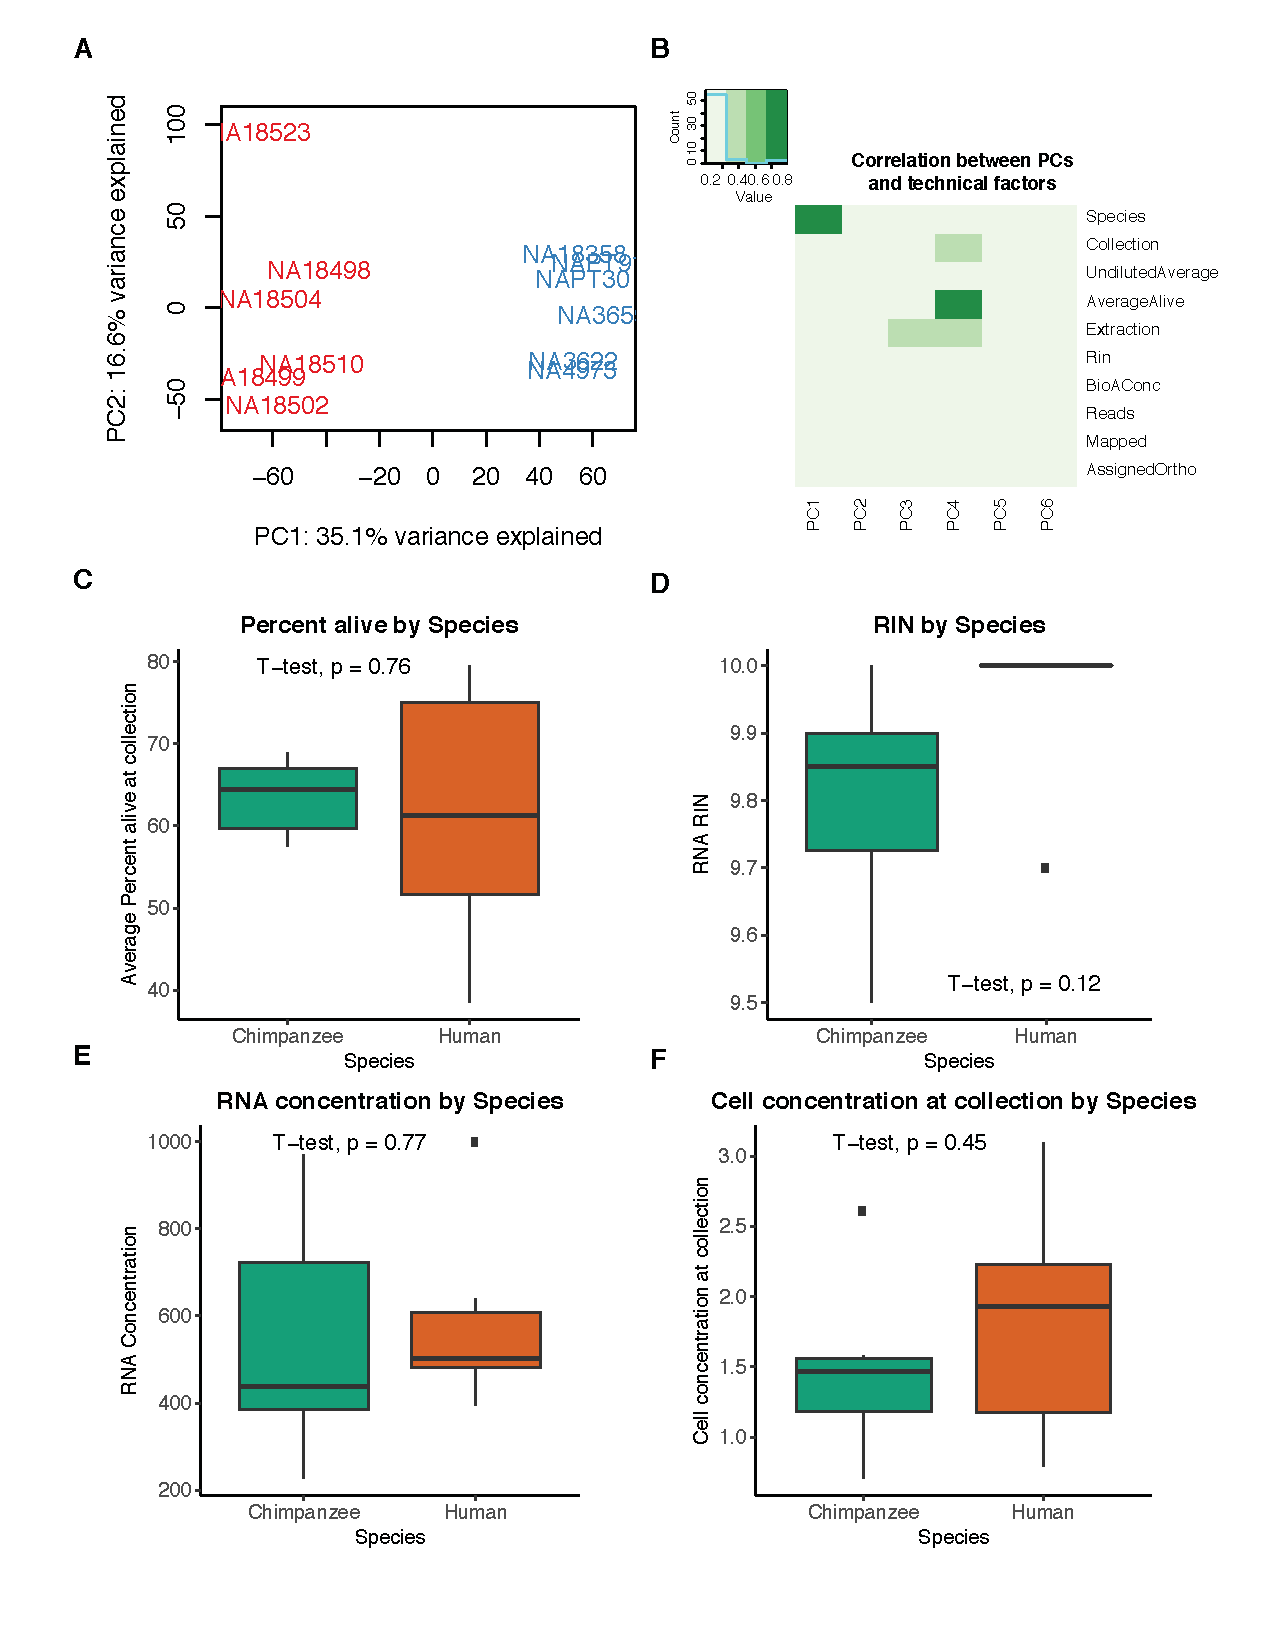
\includegraphics[width=5in]{img/ch03/Fig3_figSup4.pdf}
\caption[Differential expression quality control plots]{\textbf{Differential expression quality control plots} {\bf (A)} First two principal components \emph{(PCs)} in gene expression variation. {\bf (B)} Heatmap representing correlation between technical factors and PCs. Explanation of Y axis factors and values available in Table \ref{tab:ch03-s2} {\bf (C)} Percent of live cells as calculated by trypan blue staining at collection is not confounded by species. {\bf (D)}  RIN scores reported by bioanalyzer at RNA-seq library generation are not confounded by species.{\bf (E)}  RNA concentrations reported by bioanalyzer at RNA-seq library generation are not confounded by species. {\bf (F)}  Cell concentrations at time of collection are not confounded by species.}
\label{fig:ch03-DEQC}
\end{figure}
\clearpage


\clearpage
\section{Supplementary Tables}\label{ch03-supplementary-tables}

\begin{table}[!htb]
\caption[3' Seq metadata]{\textbf{3' Seq metadata} 
(see supplementary file associated with this dissertation) Metadata for 3' Seq data. Column names as described- Species:Cell line species , Lines: Cell line ID, Fraction: Cellular fraction, CollectionDate: Date of cell harvest and nuclear isolation, Extraction\_date: Date of RNA extraction, Collection\_person: Author initial for who processed cell harvest and nuclear isolation, UndilutedAverage: Average of 2 cell count measurements $1x10^6$, AverageAlive: Average of 2 cell live dead counts - calculated with trypan blue stain, Concentration: Extracted RNA concentration (ng/ml), RIN: RIN score for extracted RNA, 260.280.Ratio: 260/280 ratio calculated on nanodrop, Library: 3' Seq library date, Reads: Number of sequenced reads, Mapped\_wMP: Number of Mapped reads before removing reads likely due to misprimming, Mapped\_Clean: Number of Mapped reads after removing reads likely due to misprimming}
\label{tab:ch03-s1}
\end{table}


\begin{table}[!htb]
\caption[Expression Independent eQTLs]{\textbf{RNA sequencing metadata} 
(see supplementary file associated with this dissertation) Metadata for RNA sequencing data. Column names as described- Species:Cell line species , Lines: Cell line ID, Collection\_person: Author initial for who processed cell harvest and nuclear isolation, UndilutedAverage: Average of 2 cell count measurements $1x10^6$, AverageAlive: Average of 2 cell live dead counts - calculated with trypan blue stain, CollectionDate: Date of cell harvest and nuclear isolation, Extraction: Date of RNA extraction,  RIN: RIN score for extracted RNA, BioAConc: RNA concentration (ng/ul), Reads: Number of Sequenced reads, Mapped: Number of mapped reads, AssignedOrtho: Number of mapped reads assigned to orthologous exons.}
\label{tab:ch03-s2}
\end{table}

